% Capítulo 4
\chapter{Resultados}
\label{resultados}

Para cada um dos anos eleitorais analisados neste estudo são apresentados duas visualizações para o grafo gerado. Na primeira é possível identificar as comunidades encontradas pelo algoritmo de modularização, de maneira que cada comunidade possui uma cor diferente para seus vértices. Na segunda visualização do grafo cada vértice é colorido de acordo com a afinidade ideológica do partido.

Vértices em tons de vermelho são partidos de centro-esquerda, esquerda e extrema-esquerda. Vértices em tons de azul são partidos de centro-direita, direita e extrema-direita. Já os vértices verdes são os partidos que se declaram de centro, e os cinzas são partidos que não possuem uma classificação bem definida na literatura.

\subsection{Métricas gerais}
\label{proposta__objetivos-especificos--dados-gerais}

São apresentadas métricas referentes à densidade, grau médio, grau médio ponderado e modularidade, afim de facilitar a análise dos grafos gerados.


O grau médio da rede representa quantas alianças diferentes, em média, cada partido fez. Como visto na seção \ref{proposta__modelagem}, utilizamos pesos nas arestas dos grafos como forma de indicar em quantos estados os partidos em questão participam de uma mesma coligação. Assim, os grafos apresentados não indicam apenas quais são as alianças formadas, mas também o quão forte é um relacionamento entre dois partidos. O peso de cada aresta pode ser percebido na visualização dos grafos, quanto mais grossa a linha for maior o peso da aresta sendo representada.

A densidade do grafo fornece uma visão geral de como as coligações se comportam. Isto é, uma componente muito densa indica que os partidos fazem muitas alianças diferentes, portanto a afinidade ideológica tem pouca influência na formação destas coligações.

%%%%%%%%%%%%%%%%%%%%%%%%%%%%%%%%%%%%%%%%%%%%%%%%%%%%%%%%%%%
\section{\texorpdfstring{\MakeUppercase{Parâmetros para modularização}}{}}
\label{resultados__parametros-modularizacao}

Para a utilização do algoritmo de detecção de comunidades é necessário escolher um parâmetro de \emph{resolução}, quanto maior o valor deste parâmetro menos comunidades são geradas.

Assim, utilizamos o valor de resolução 1,2 para os grafos de 1994, 1998, 2002 e 2006. Com este parâmetro, o algoritmo de modularização conseguiu separar a componente gigante dos grafos em duas comunidades. Para os anos 2010 e 2014 percebeu-se a necessidade de reduzir o valor de resolução para 1,0, uma vez que ao utilizar 1,2 como parâmetro a componente gigante se tornava uma única comunidade (mais detalhes nas seções \ref{resultados__grafos--2010} e \ref{resultados__grafos--2014}).

%%%%%%%%%%%%%%%%%%%%%%%%%%%%%%%%%%%%%%%%%%%%%%%%%%%%%%%%%%%
\section{\texorpdfstring{\MakeUppercase{Grafos}}{}}
\label{resultados__grafos}
%% Gráficos, números, conclusões: como as comunidades ficaram, grau médio, coeficiente de clustering


\subsection{1994}
\label{resultados__grafos--1994}

\begin{figure}[H]
\center
    \subfigure[fig-1994][Comunidades $C_0$ (vértices rosas) e $C_1$ (vértices verdes)]{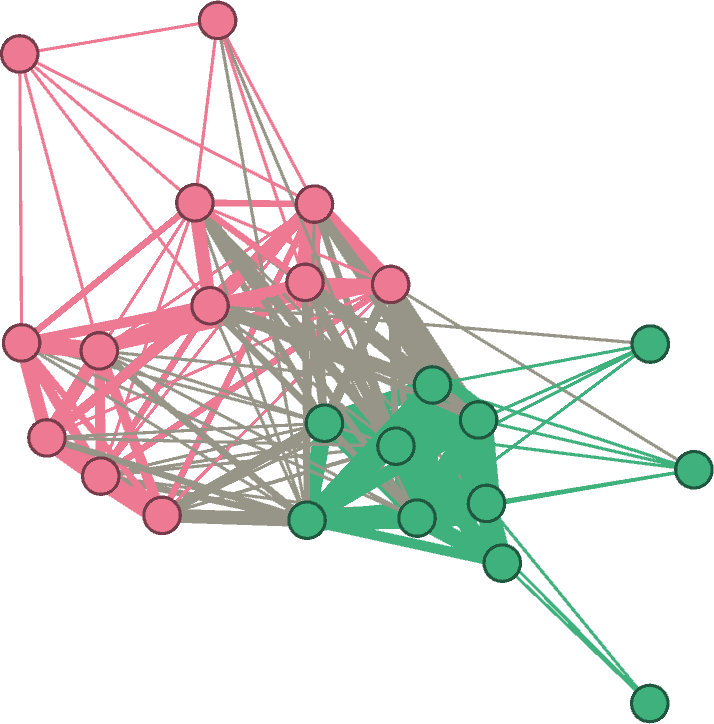
\includegraphics[width=7.5cm]{img/grafos/1994a.png}\label{fig:grafos-1994-a}}
    \qquad
    \subfigure[fig-1994b][Eixo político dos partidos]{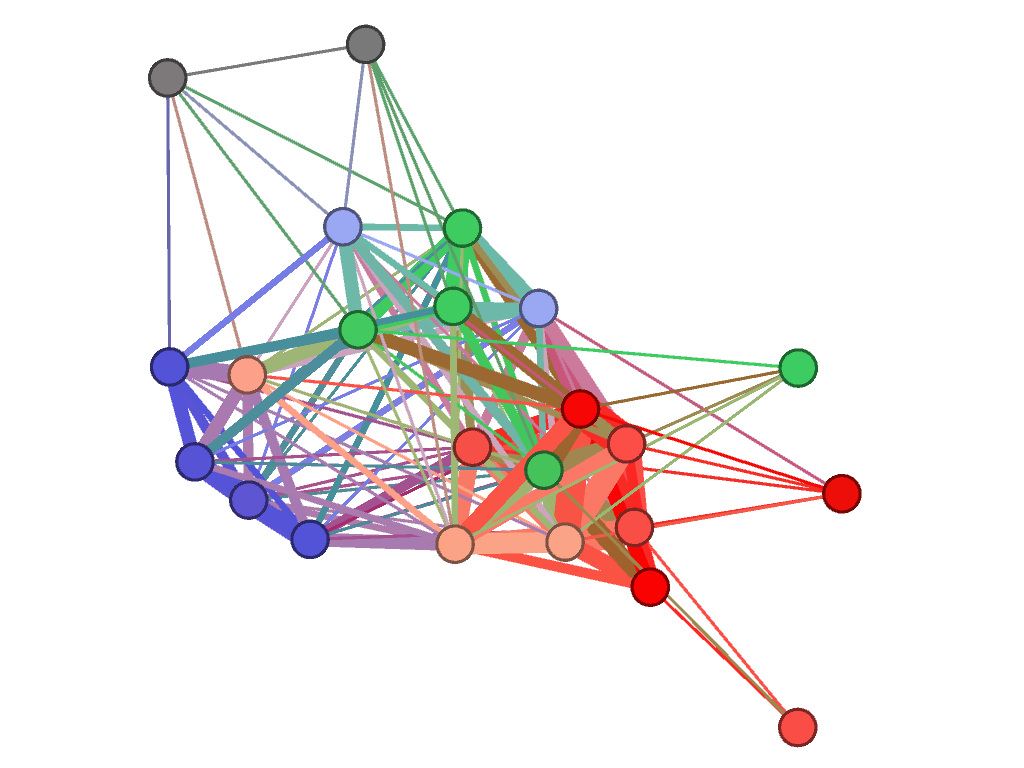
\includegraphics[width=7.5cm]{img/grafos/1994c.png}}
    
    \caption{1994: Comunidades e espectro político}
\end{figure}

Ao comparar as duas visualizações do grafo de 1994 podemos perceber que as duas comunidades geradas, $C_0$ e $C_1$, possuem uma divisão evidente na afinidade ideológica de seus partidos. A Tabela \ref{table-1994} apresenta algumas métricas gerais do grafo. Observando a quantidade de vértices, nota-se que a divisão de grupos foi bem balanceada, $C_0$ e $C_1$ contendo 12 e 11 vértices respectivamente.

\begin{table}[H]
\centering
\begin{tabular}{|l|l|l|l|}
\hline
Total de arestas  & 142 & Modularidade         & 0,230 \\ \hline
Total de vértices & 23   & Grau Médio           & 12,348 \\ \hline
Vértices em $C_0$    & 12 (52,17\%)  & Grau Médio Ponderado & 33,043 \\ \hline
Vértices em $C_1$    & 11 (47.83\%) & Densidade            &  0,561\\ \hline
\end{tabular}
\caption{Métricas do grafo de coligações em 1994}
\label{table-1994}
\end{table}

Ressalta-se que esta divisão dos vértices não significa que partidos da esquerda só fazem aliança com partidos de mesma ideologia por exemplo. As arestas dos grafos tendem a manter a cor dos vértices em que elas incidem, mas na figura \ref{fig:grafos-1994-a} podemos ver uma grande quantidade de arestas cinzas, que apresentam esta cor por conectar vértices rosas e verdes. Isto significa que existem várias alianças sendo feitas entre os partidos das duas comunidades opostas.

Percebe-se ainda que os partidos sem classificação ideológica (\gls{PRN} e \gls{PTRB}, vértices cinzas) ficaram nas extremidades do grafo, indicando que possuem grau menor em relação aos demais vértices e, portanto, fizeram menos alianças, assim como os vértices - \gls{PCB}, \gls{PTdoB} e \gls{PRONA} - nas extremidades da comunidade C1.


\subsection{1998}
\label{resultados__grafos--1998}

\begin{figure}[H]
\center
    \subfigure[fig-1998][Comunidades $C_0$ (vértices em laranja) e $C_1$ (vértices verdes)]{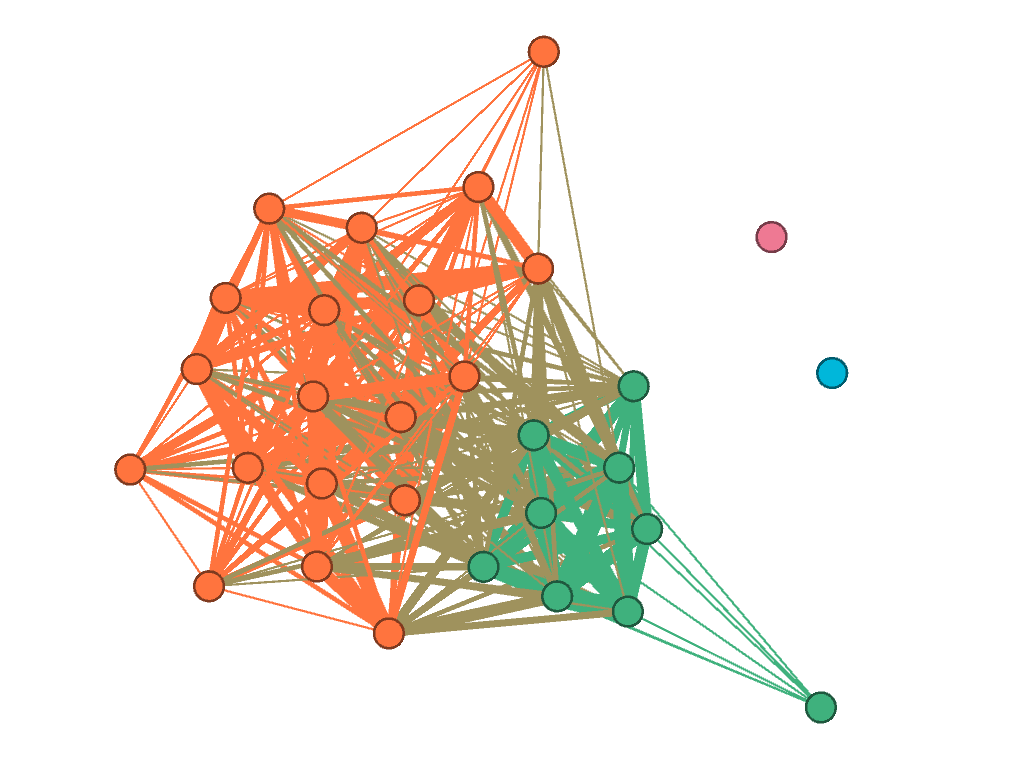
\includegraphics[width=7.5cm]{img/grafos/1998a.png}}
    \qquad
    \subfigure[fig-1998b][Eixo político dos partidos]{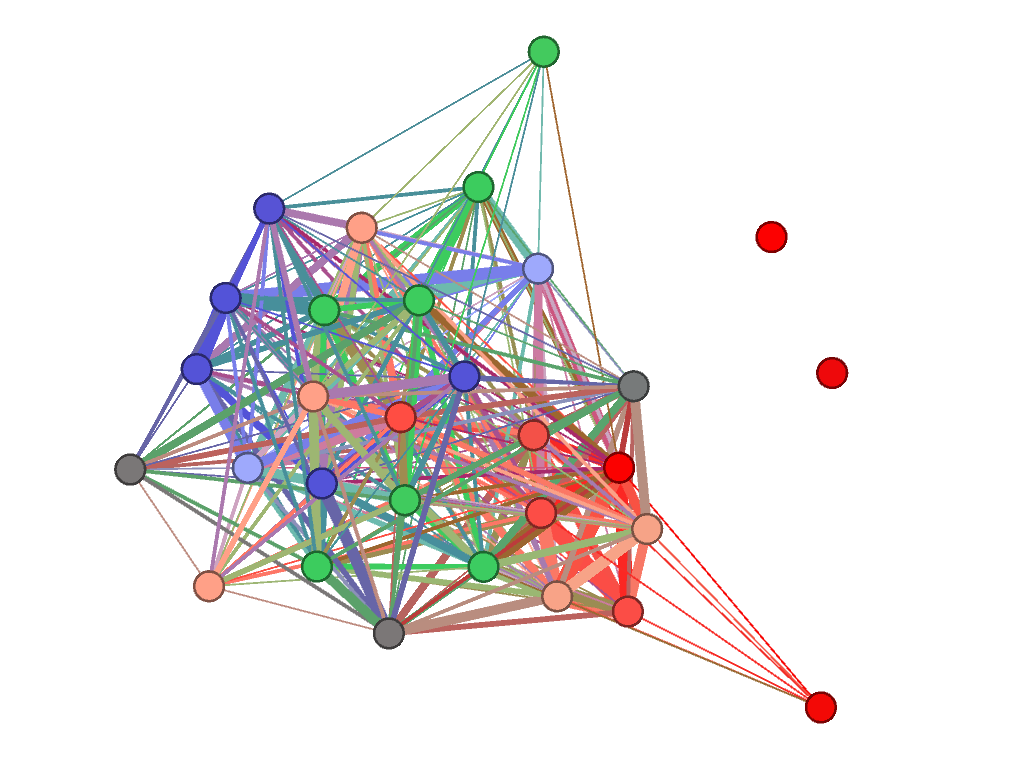
\includegraphics[width=7.5cm]{img/grafos/1998c.png}}
    
    \caption{1998: Comunidades e espectro político}
\end{figure}

Percebe-se que o grafo gerado para 1998 não é conexo, contendo dois vértices sem arestas. Isso indica que existem dois partidos que não se coligaram em nenhum estado do Brasil nesse ano (\gls{PCO} e \gls{PSTU}). Estes vértices não são considerados comunidades, mas optamos por manter no grafo para uma melhor visualização do comportamento geral de todos os partidos. Identificam-se ainda três partidos de centro-esquerda e um de esquerda - \gls{PTdoB}, \gls{PGT}, \gls{PTB} e \gls{PST} - na comunidade $C_0$, que tem predominância de legendas de direita.

A divisão dos partidos de esquerda e direita nas duas comunidades manteve-se neste ano, apesar de não ser tão evidente quanto em 1994. Isso se dá, em parte, ao fato de que o grafo é mais denso, como mostrado na Tabela \ref{table-1998}. 



\begin{table}[H]
\centering
\begin{tabular}{|l|l|l|l|}
\hline
Total de arestas  & 295 & Modularidade         & 0,161 \\ \hline
Total de vértices & 30  & Grau Médio           & 19,667 \\ \hline
Vértices em $C_0$    & 19  (63,33\%) & Grau Médio Ponderado & 50,533 \\ \hline
Vértices em $C_1$    & 9 (30\%) & Densidade            &  0,678\\ \hline
\end{tabular}
\caption{Números absolutos e relativos do grafo de coligações em 1998}
\label{table-1998}
\end{table}

Embora este grafo apresente apenas dois vértices a mais do que em 1994, o número de arestas aumentou consideravelmente: 295 em 1998, mais do que o dobro de arestas em 1994, indicando um crescimento expressivo na quantidade de alianças feitas.


\subsection{2002}
\label{resultados__grafos--2002}

\begin{figure}[H]
\center
    \subfigure[fig-2002][Comunidades $C_0$ (vértices em rosa) e $C_1$ (vértices verdes)]{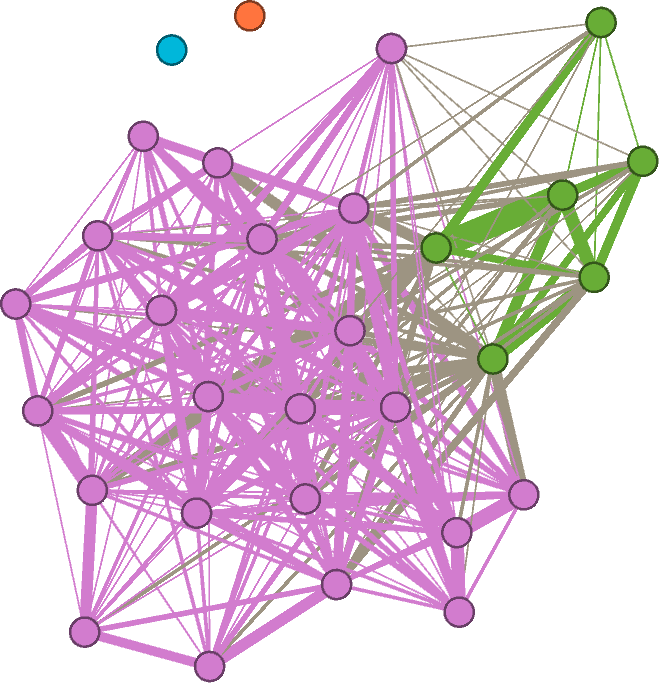
\includegraphics[width=7.5cm]{img/grafos/2002a.png}}
    \qquad
    \subfigure[fig-2002b][Espectro político dos partidos]{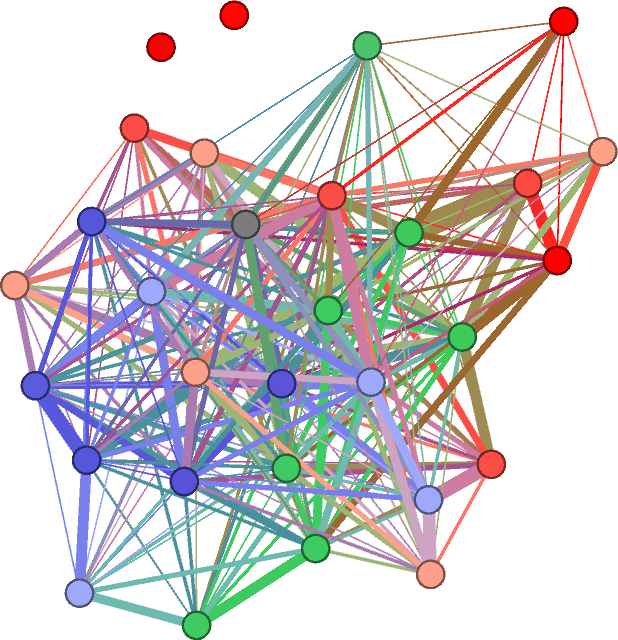
\includegraphics[width=7.5cm]{img/grafos/2002c.png}}
    
    \caption{2002: Comunidades e espectro político}
\end{figure}

Em 2002 percebe-se a existência de uma discrepância maior no tamanho das comunidades. A menor possui 6 partidos (eram 11 em 1994), fazendo com que o \emph{cluster} $C_0$ contenha 73,33\% dos vértices do grafo, como mostra a Tabela \ref{table-2002}. Apesar do tamanho reduzido, $C_1$ continua apresentando uma certa predominância ideológica: não contém nenhum partido de direita, sendo composta majoritariamente por legendas de esquerda.

Nota-se também que existem partidos de centro-esquerda em $C_0$, na qual a maioria é de direita. Este agrupamento contém novamente grande parte dos partidos centristas (5 dos 7 presentes no grafo). 

\begin{table}[H]
\centering
\begin{tabular}{|l|l|l|l|}
\hline
Total de arestas  & 269 & Modularidade         & 0,101 \\ \hline
Total de vértices & 30  & Grau Médio           & 17,933 \\ \hline
Vértices em $C_0$    & 22  (73,33\%) & Grau Médio Ponderado & 47,733 \\ \hline
Vértices em $C_1$    & 6 (20\%) & Densidade            &  0,618\\ \hline
\end{tabular}
\caption{Números absolutos e relativos do grafo de coligações em 2002}
\label{table-2002}
\end{table}

\subsection{2006}
\label{resultados__grafos--2006}

\begin{figure}[H]
\center
    \subfigure[fig-2006][Comunidades $C_0$ (vértices em rosa), $C_1$ (vértices verdes) e $C_2$ (vértices cinzas)]{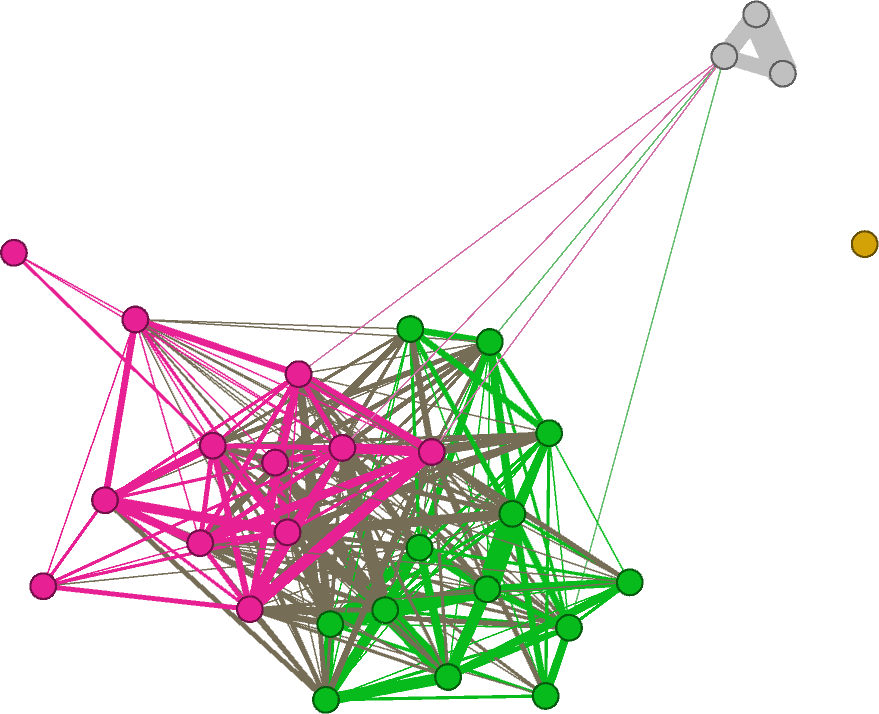
\includegraphics[width=7.5cm]{img/grafos/2006a.png}}
    \qquad
    \subfigure[fig-2006b][Espectro político dos partidos]{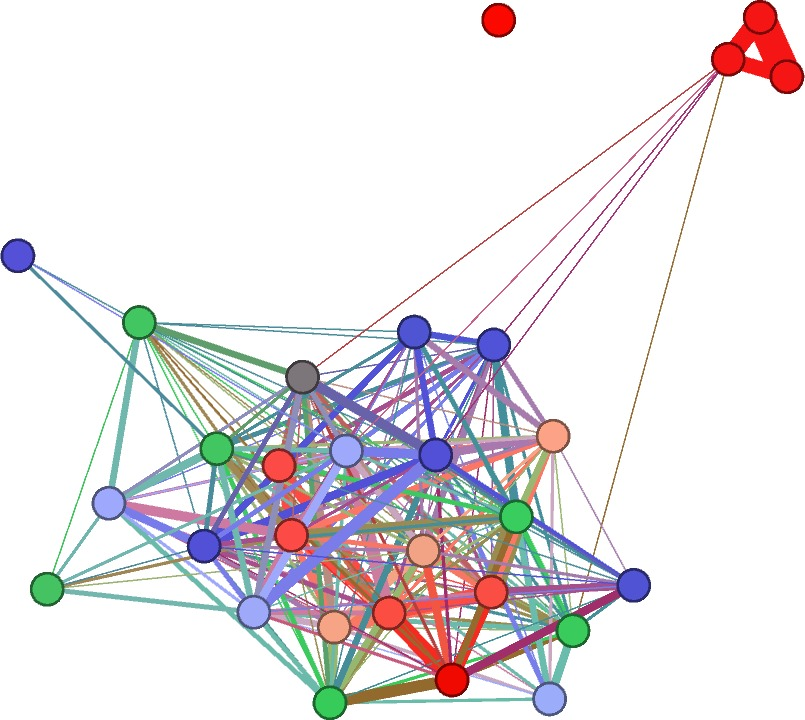
\includegraphics[width=7.5cm]{img/grafos/2006c.png}}
    
    \caption{2006: Comunidades e espectro político}
\end{figure}

Neste ano são identificadas três comunidades na componente principal e o tamanho das duas comunidades maiores voltou a ser mais equilibrado. O novo \emph{cluster}, $C_2$, está posicionado longe dos demais vértices, indicando que o número de conexões destes partidos com  os demais é pequeno. Esta comunidade contém três partidos (vide Tabela \eqref{table-2006a}) de extrema-esquerda: \gls{PCB}, \gls{PSOL} e \gls{PSTU}, e sua separação dos demais vértices nos indica que estes partidos (de ideologias muito bem definidas) costumam fazer poucas ou nenhuma aliança com os demais. Entre os três, o único a se aliar com partidos das outras comunidades é o \gls{PCB}. Chamamos a atenção para o fato de que uma destas alianças é com o \gls{PSC}, partido que historicamente se opõe aos ideais comunistas, que são fortemente presentes nas pautas do partido esquerdista.

\begin{table}[H]
\centering
\begin{tabular}{|l|l|}
\hline
Comunidade & Vértices \\ \hline
$C_0$         &      12 (48,48\%)                \\ \hline
$C_1$         &     13 (39,39\%)                \\ \hline
$C_2$         &       3 (9,09\%)               \\ \hline
\end{tabular}
\caption{Tamanho das comunidades em 2006}
\label{table-2006a}
\end{table}

A distinção entre esquerda e direita torna-se menos presente neste grafo, a comunidade $C_1$ por exemplo, contém legendas de diversas afinidades ideológicas: \gls{PSDB}, \gls{PT}, \gls{PMDB}, \gls{PCdoB}, \gls{PP} e \gls{PL}. Entre os anos utilizado neste estudo, 2006 é o que apresenta o grafo menos denso, como mostrado na Tabela \ref{table-2006b}.

\begin{table}[H]
\centering
\begin{tabular}{|l|l|l|l|}
\hline
Total de arestas  & 222 & Grau Médio           & 15,31 \\ \hline
Total de vértices & 29 & Grau Médio Ponderado & 43,103 \\ \hline
Modularidade      & 0,196 & Densidade            & 0,547 \\ \hline
\end{tabular}
\caption{Números absolutos do grafo de coligações em 2006}
\label{table-2006b}
\end{table}

\subsection{2010}
\label{resultados__grafos--2010}

\begin{figure}[H]
\center
    \subfigure[fig-2010][Comunidades $C_0$ (roxo), $C_1$ (marrom), $C_2$ (vermelho), $C_3$ (verde) e $C_4$ (rosa)]{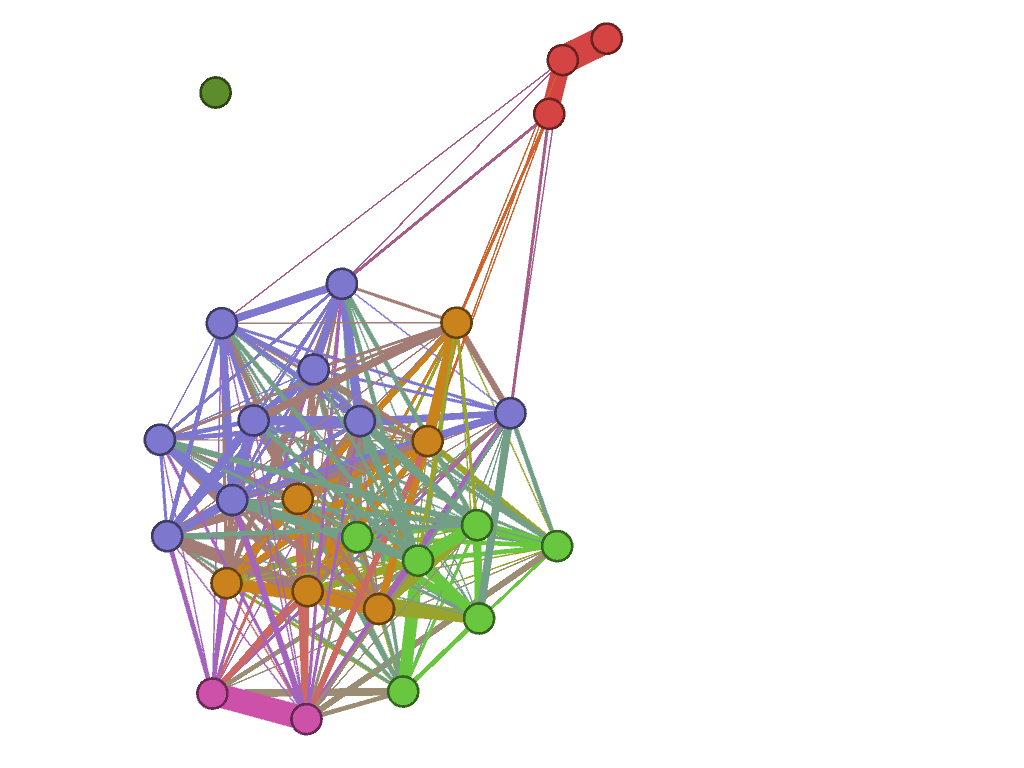
\includegraphics[width=7.5cm]{img/grafos/2010a.png}}
    \qquad
    \subfigure[fig-2010b][Espectro político dos partidos]{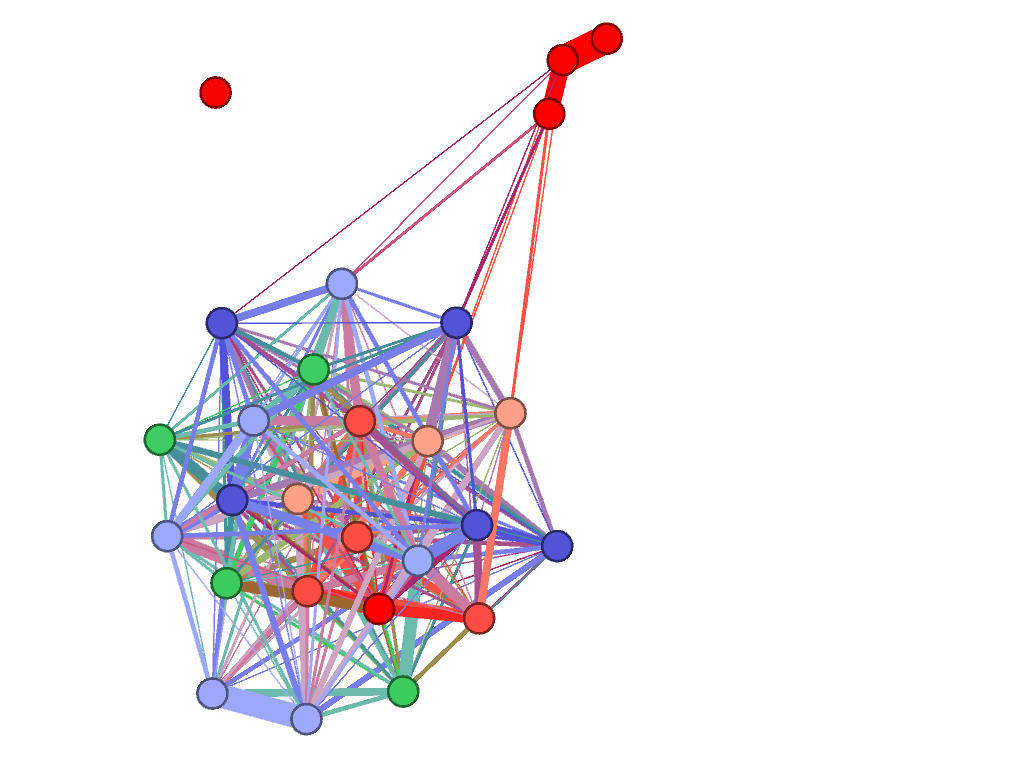
\includegraphics[width=7.5cm]{img/grafos/2010c.png}}
    
    \caption{2010: Comunidades e espectro político}
\end{figure}

Em 2010 foi necessário mudar a resolução, ao utilizar 1,2 como parâmetro não foi possível separar a componente principal em duas comunidades (ou três, como em 2006). Isso se dá, em parte, porque o grafo gerado para este ano é muito mais denso do que nos anos anteriores, como mostrado na Tabela \ref{table-2010a}. Esta densidade é perceptível visualmente no grafo: os vértices estão muito próximos com uma quantidade grande de arestas entre eles. 

\begin{table}[H]
\centering
\begin{tabular}{|l|l|l|l|}
\hline
Total de arestas  & 245 & Grau Médio           & 18,148 \\ \hline
Total de vértices & 27 & Grau Médio Ponderado & 52,889 \\ \hline
Modularidade      & 0,158 & Densidade            & 0,698 \\ \hline
\end{tabular}
\caption{Números absolutos do grafo de coligações em 2010}
\label{table-2010a}
\end{table}

Assim, ao aplicar o algoritmo de modularidade com resolução menor obteve-se um número maior de comunidades, como mostrado na Figura \ref{resultados__grafos--2010} (a) e na Tabela \ref{table-2010b}. Chamamos atenção para a comunidade de cor rosa que conecta apenas dois vértices: \gls{PSDB} e \gls{DEM}. A separação de uma comunidade com apenas estes dois partidos ocorreu pois o grau da aresta que os conecta é 15, indicando que esta aliança ocorreu em 15 estados brasileiros, sendo assim o segundo maior peso do grafo, atrás apenas da aliança \gls{PSTU} e \gls{PSOL}, que ocorreu em 18 estados.

\begin{table}[H]
\centering
\begin{tabular}{|l|l|}
\hline
Comunidade & Vértices \\ \hline
$C_0$         &     9 (33,33\%)                \\ \hline
$C_1$         &     6 (22,22\%)                \\ \hline
$C_2$         &       3 (11,11\%)               \\ \hline
$C_3$         &       6 (22,22\%)               \\ \hline
$C_4$         &       2 (7,4\%)               \\ \hline
\end{tabular}
\caption{Tamanho das comunidades em 2010}
\label{table-2010b}
\end{table}

O aumento de comunidades e densidade no grafo dificulta a identificação das ideologias predominantes em cada agrupamento, o que evidencia a redução (em relação aos anos anteriores) de afinidade ideológica presente nas coligações formadas em 2010.

%%%%%
\subsection{2014}
\label{resultados__grafos--2014}

\begin{figure}[H]
\center
    \subfigure[fig-2014][Comunidades identificadas]{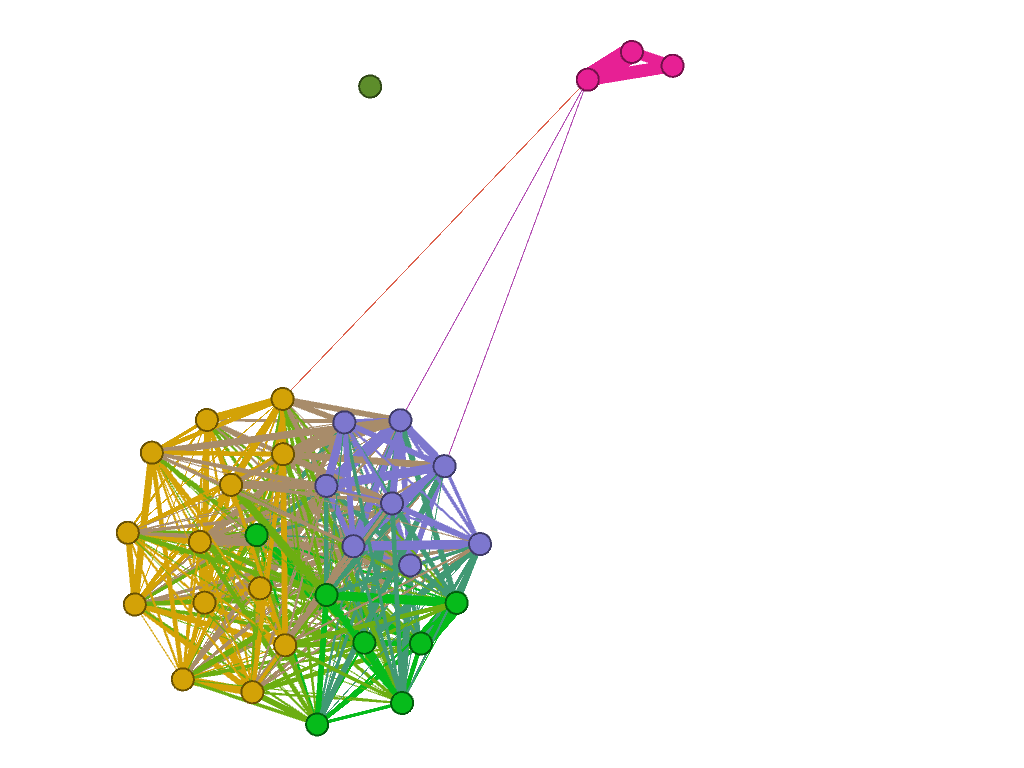
\includegraphics[width=7.5cm]{img/grafos/2014a.png}}
    \qquad
    \subfigure[fig-2014b][Espectro político dos partidos]{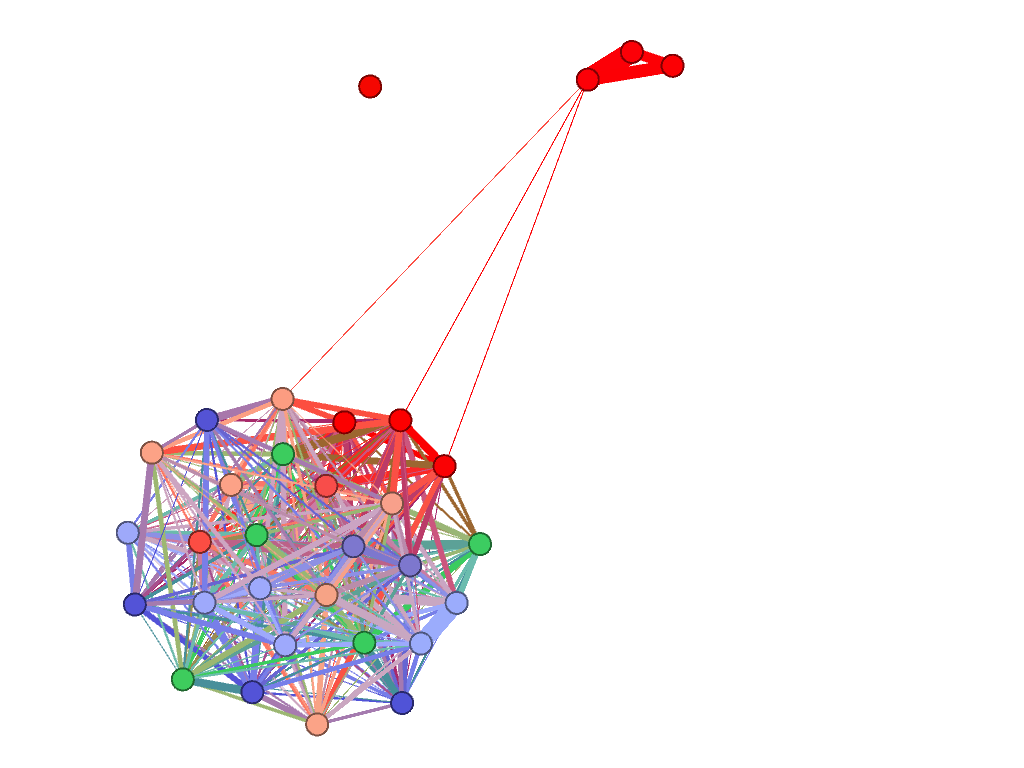
\includegraphics[width=7.5cm]{img/grafos/2014c.png}}
    
    \caption{2014: Comunidades e espectro político}
\end{figure}

\todo{Este grafo vai ser corrigido, está com um erro de cor em alguns vértices}

Para este grafo também foi necessário utilizar o valor 1,0 como resolução, implicando na identificação de quatro comunidades, como mostra a Tabela \ref{table-2014a}. Ele é ainda mais denso que os anteriores e apresenta o maior número de arestas até então (vide Tabela \ref{table-2014b}, o que é perceptível visualmente. Novamente uma comunidade com partidos de extrema-esquerda é formada, sendo assim o único agrupamento de vértices distantes do restante do grafo. 
\begin{table}[H]
\centering
\begin{tabular}{|l|l|}
\hline
Comunidade & Vértices \\ \hline
$C_0$         &     13 (40,62\%)                \\ \hline
$C_1$         &     8 (25\%)                \\ \hline
$C_2$         &       3 (9,37\%)               \\ \hline
$C_3$         &       7 (21,87\%)               \\ \hline
\end{tabular}
\caption{Tamanho das comunidades em 2014}
\label{table-2014a}
\end{table}


\begin{table}[H]
\centering
\begin{tabular}{|l|l|l|l|}
\hline
Total de arestas  & 356 & Grau Médio           & 22,25 \\ \hline
Total de vértices & 32 & Grau Médio Ponderado & 69,25 \\ \hline
Modularidade      & 0,138 & Densidade            & 0,718 \\ \hline
\end{tabular}
\caption{Números absolutos do grafo de coligações em 2014}
\label{table-2014b}
\end{table}

Na Figura \ref{resultados__grafos--2014} (b) percebe-se que de forma geral os vértices vermelhos e azuis se encontram em regiões opostas, dando a impressão de que existe um tipo de separação por ideologia, mas isso não reflete necessariamente a realidade. O aumento na densidade do grafo e a necessidade de alterar o valor de resolução do algoritmo  de modularidade (mesmo assim não sendo possível separar o grafo em duas comunidades) indicam um aumento no número de alianças entre partidos de ideologias diferentes. 

%%%%%%%%%%%%%%%%%%%%%%%%%%%%%%%%%%%%%%%%%%%%%%%%%%%%%%%%%%%
\section{\texorpdfstring{\MakeUppercase{Gráficos Gerais}}{}}
\label{resultados__graficos-gerais}

A seguir são apresentados gráficos que facilitam uma análise geral das coligações partidárias ao longo dos anos. 

\begin{figure}[H]
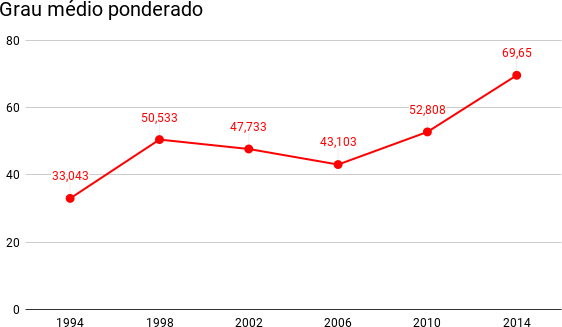
\includegraphics[width=1\textwidth]{4-resultados/graficos/graumedioponderado.png}
\centering
\caption{
    Grau médio ponderado dos grafos ao longo dos anos
}
\label{fig:grafico-graumedioponderado}
\end{figure}

A Figura \ref{fig:grafico-graumedioponderado} apresenta o grau médio ponderado dos grafos. Percebe-se que os dois anos com os menores valores são 1994 - isso é visível até mesmo no grafo, que contém muito menos arestas em relação aos demais -  e 2006.

Em 2010 este número voltou a aumentar, e atingiu seu maior valor até então em 2014. Neste ano cada partido fez, em média, quase 70 alianças em todo o Brasil. 

Como o número de partidos (Figura \ref{fig:grafico-verticesarestas}) quase não mudou ao longo dos anos, o crescimento no valor do grau médio indica que a quantidade de alianças feitas entre as diferentes legendas tem aumentado, e consequentemente a afinidade ideológica é um fator cada vez menos influente nas coligações.

\begin{figure}[H]
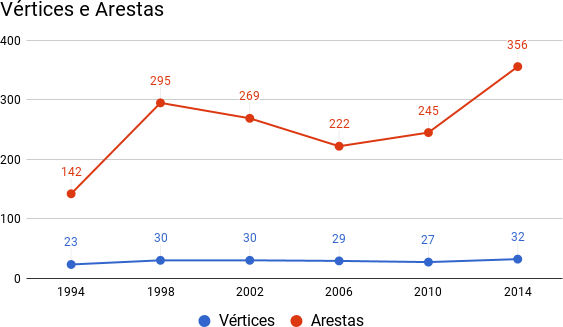
\includegraphics[width=1\textwidth]{4-resultados/graficos/vertices-arestas.png}
\centering
\caption{
    Grau médio dos grafos ao longo dos anos
}
\label{fig:grafico-verticesarestas}
\end{figure}

Ao analisar o gráfico de vértices e arestas, percebe-se que embora a quantidade de vértices permaneça quase inalterada (a única exceção é em 1994, com o menor número de partidos, 24), o total de arestas varia consideravelmente.


A Figura \ref{fig:grafico-comunidades} permite uma visão mais ampla da distribuição de ideologia das legendas em cada comunidade encontrada nos grafos.

\begin{figure}[H]
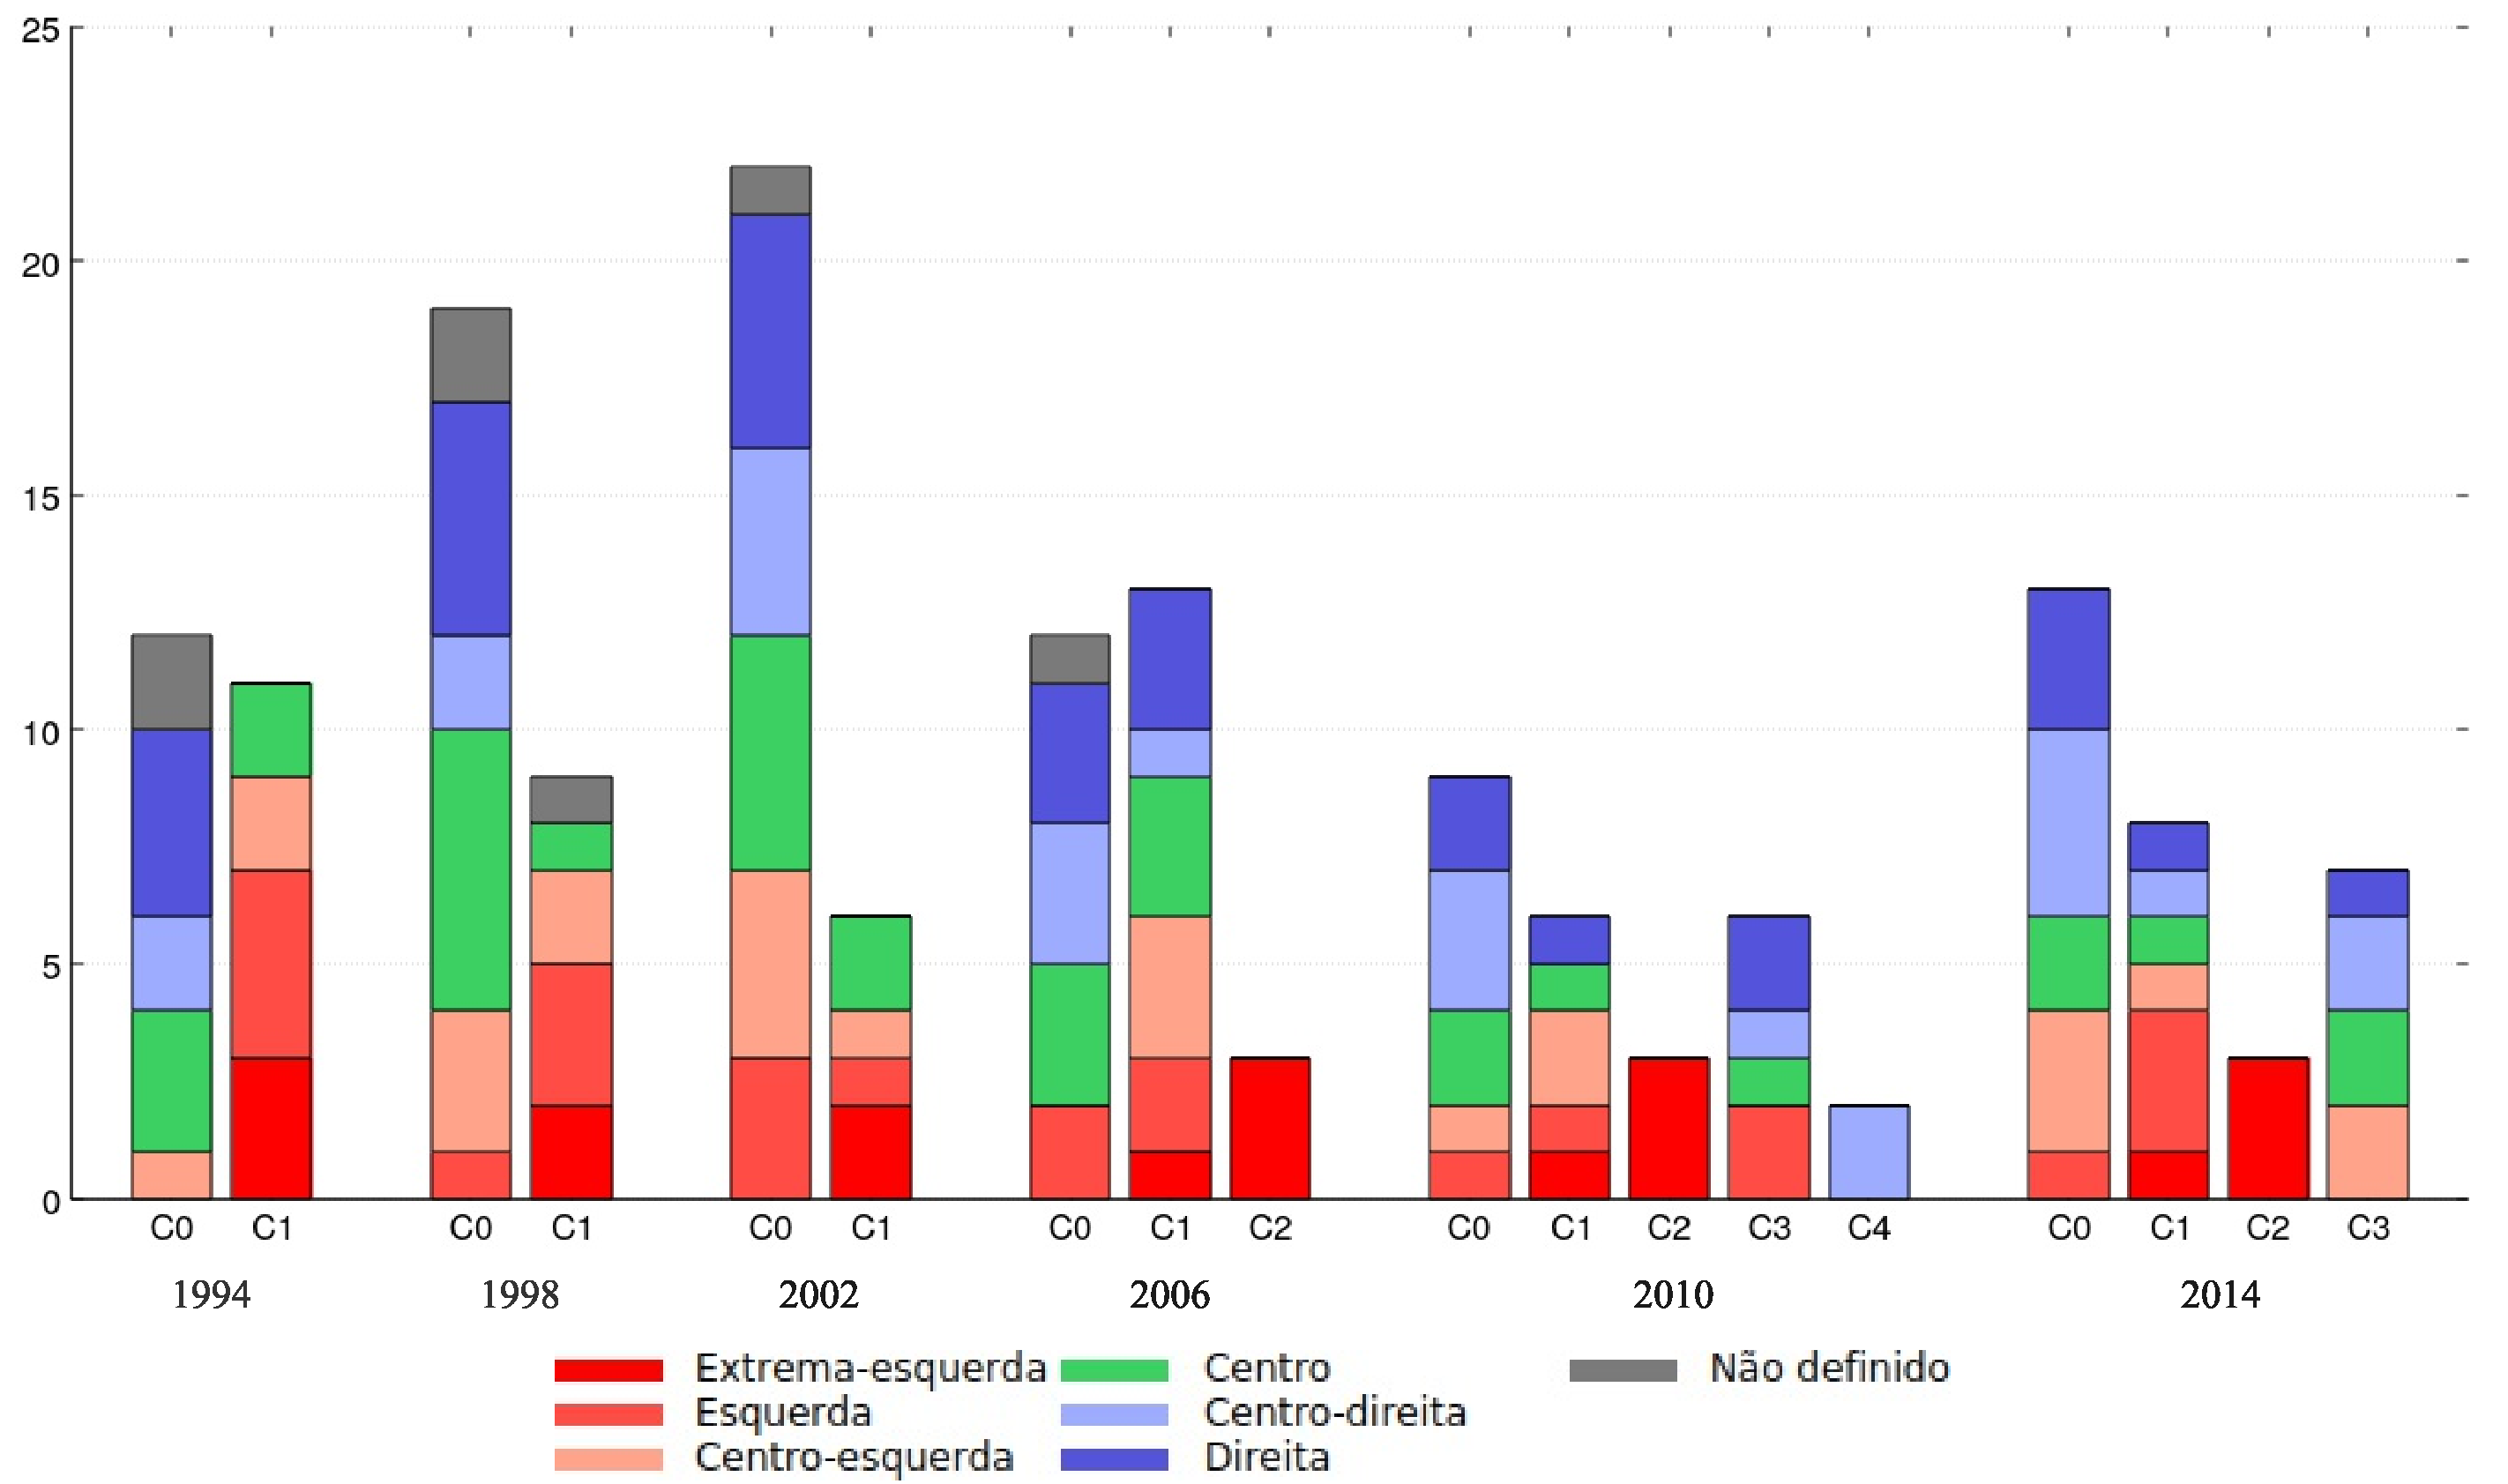
\includegraphics[width=1\textwidth]{4-resultados/graficos/grafico-geral.pdf}
\centering
\caption{
    Gráfico de distribuição de ideologia das coligações
}
\label{fig:grafico-comunidades}
\end{figure}


Analisando o gráfico é possível perceber que para os anos 1994 e 1998 as comunidades apresentavam uma distinção clara de afinidade ideológica dos seus partidos, indicando que nestes anos as coligações foram formadas no geral por legendas de ideologias parecidas. Isso deixou de ocorrer ao longo dos próximos anos, o número de alianças entre partidos diversos aumentou e as comunidades começaram a apresentar mais diversidade ideológica.

